\documentclass{article}
\usepackage[utf8]{inputenc}
\usepackage{amsmath,amssymb}
\usepackage{paralist}
\usepackage{color}
\usepackage[detect-weight=true, binary-units=true]{siunitx}
\usepackage{pgfplots}
\usepackage{authblk}
\usepackage{url}
\usepackage{multirow}
\usepackage{booktabs}
\usepackage{inconsolata}
\usepackage{caption}
\captionsetup{tableposition=top,figureposition=bottom,font=small,format=hang,labelfont={sf,bf}}
\usepackage{graphicx}
\usepackage{tabularx}
\usepackage{listings}
\usepackage{hyphenat}
\usepackage{subfig}
\usepackage{float}
\pagestyle{empty}
\usepackage{hyperref}
\hypersetup{
  colorlinks   = true, %Colours links instead of ugly boxes
  urlcolor     = black, %Colour for external hyperlinks
  linkcolor    = black, %Colour of internal links
  citecolor   = black %Colour of citations
}

\title{Machine Learning and Data Mining project:\\Predicting NBA playoff results}
\author{Silvio Angelo Baratto Roldan}
\date{Course of AA $2021$-$2022$ - Data Science and Scientific Computing}



\begin{document}

\maketitle

\begin{abstract}
The NBA playoffs are part of the NBA-related league. This competition consists of four rounds between eight Eastern Conference and Western Conference teams. The playoffs are made up in the eights, quarter-finals, semifinals and final of the Conference. Finally, the winners of each final of their conference clash with the other winner in the NBA Finals. Each round consists of 7 games, so it takes 4 games to win to move on to the next round.
\end{abstract}
\section{Problem statement}
\label{section: ProblemStatement}
The goal of this project is to create a model [\ref{fig:modelExplain}] that simulates the complete playoff scoreboard and predicts the winner of each game and round. The model is composed by three parts: training the model, generating feature values and simulation.
\section{Assessment and performance indexes}
\label{section: AssesmentPerformanceIndexes}
To select the best classifier to train the model and to use it in the simulations three different metrics have been taken in consideration:
\begin{itemize}
\item{\texttt{Accuracy}}: Accuracy it is defined as the number of true positives and true negatives divided by the number of true positives, true negatives, false positives, and false negatives.
\begin{equation}
Accuracy = \dfrac{TP + TN}{TP + TN + FP + FN}
\end{equation}
\item{\texttt{AUC}}: The Receiver Operator Characteristic (ROC) curve is an evaluation metric for binary classification problems. It is a probability curve that plots the TPR (True Positive Rate) against FPR (False Positive Rate) at various threshold values and essentially separates the ‘signal’ from the ‘noise’. The Area Under the Curve is the measure of the ability of a classifier to distinguish between classes and is used as a summary of the ROC curve. The higher the AUC, the better the performance of the model at distinguishing between the positive and negative classes.
\item{\texttt{MSE}}: Measures of the averages of the squares of the errors that is, the average squared difference between the estimated values and the actual value.
\begin{equation}
MSE = \dfrac{\sum_{i = 1}^n (x_i - \hat{x_i})^2}{n}
\end{equation}
\end{itemize}
\section{Proposed solution}
\label{section: ProposedaSolution}
For the purpose of simulation high accuracy and low error were the goals when selecting the right model. At this purpose three different classifier have been taken in consideration. In the table below [\ref{tab:modelComparison}] is show the Pros e Cons between them
\begin{table}[H]
	\centering
	\begin{tabular}{l|l|l|l|l}
	\toprule
	Model 			& interpretable 	& Accuracy 		& Training speed 	& Prediction speed	\\
    \midrule
    SVM				& No				& Higher							& Fast				& Fast				\\
    \midrule
    Random Forest 	& No				& Higher							& Slow				& Slow				\\
    \midrule
    Naive Bayes		& Moderate			& Lower								& Fast				& Fast          	\\
	\bottomrule
	\end{tabular}
\caption{Pros e Cons between SVM, Random Forest and Naive Bayes}
\label{tab:modelComparison}
\end{table}
\section{Experimental evaluation}
\label{section: ExperimentalEvaluation}
\subsection{Data}
The complete dataset was composed by 5 .csv files:
\begin{itemize}
\item \texttt{games.csv} : all games from 2004 season to last update with the date, teams and some details like number of points, etc.
\item \texttt{games\_details.csv} : details of games dataset, all statistics of players for a given game.
\item \texttt{players.csv} : players details (name).
\item \texttt{ranking.csv} : ranking of NBA given a day.
\item \texttt{teams.csv} : all teams of NBA. 
\end{itemize}
To train the model, only the data present in the games and teams dataset were used. The variables used within the \texttt{games.csv} dataset are: field goal percentage, field goal three point percentage, free throws made, rebounds, assists, steals and blocks from January 2004 untill march 2021 both for the home and visitor teams. 
\subsection{Procedure}
\label{section: Procedure}
The model consists of three parts:
\begin{itemize}
\item {\textbf{ML model selection}}: Initially, the data is analyzed and trained with a regression model to predict the probability of winning. 
\item {\textbf{Generate feature values}}: To simulate the playoffs, feature data were artificially generated with the use of different statistical distributions. For this purpose, the most recent data in \texttt{games.csv} were used to generate new data, as they are more representative.
\item {\textbf{Simulate playoff}}: Using the generated data, multiple game simulations are done. The winner of each game is predicted using the trained model. The final simulation result is the average of the simulation results.
\end{itemize}
\begin{figure}[H]
    \centering
    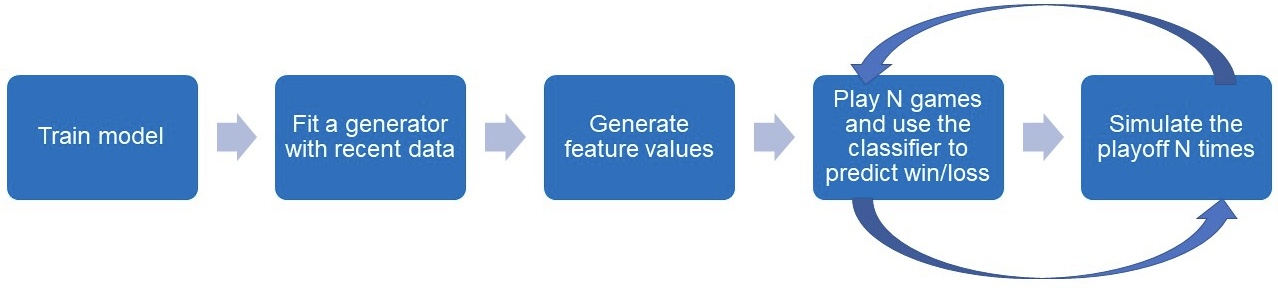
\includegraphics[width=\textwidth]{model/explain.jpeg}
    \caption{Flow diagram}
    \label{fig:modelExplain}
\end{figure}
\subsection{Results and discussion}
\label{ResultsAndDiscussion}
In the project, the selection of the right classification model is central to the correct forecast of the scoreboard. In the section [\ref{section: ProposedaSolution}] the benefits of the three models chosen for the simulations have been listed. The table [\ref{tab:results}] shows the results:
\begin{table}[H]
	\centering
	\begin{tabular}{c|c|c|c}
	\toprule
	& SVM & Random Forest & Naive Bayes\\
    \midrule
    Accuracy & $0.71$ & $0.84$ & $0.83$ \\
    \midrule
    AUC & $0.71$ & $0.83$ & $0.82$ \\
    \midrule
    MSE & $0.28$ & $0.16$ & $0.16$ \\
    \midrule
    Time & 1min, 15sec & 31min, 27sec & 51 sec \\
	\bottomrule
	\end{tabular}
\caption{Metrics results}
\label{tab:results}
\end{table}
\indent As you can see from table [\ref{tab:results}] Random Forest and Naive Bayes result the best models for both accuracy and average error. From table [\ref{tab:modelComparison}] we expected Naive Bayes perform worse than SVM but both models are sensitive to parameter optimization, without tuning the hyperparametres SVM performs better than Naive Bayes. Random Forest result the most accurate classifier. Despite this, in the game simulation the execution times for 5000 iterations were extremely higher for Random Forest compared to Naive Bayes and SVM. However, for the correct forecast of the scoreboard, the waiting time necessary for the simulation is not considered an essential metric, as the model predicts the result before the event of the playoffs and therefore does not require a forecast rate in real time. In conclusion, Random Forest is the model that is considered most appropriate to use to predict the final scoreboard. 
\subsubsection{Model output}
The figure below shows the output achieved after 5000 simulations of the playoffs of the current season 2021-2022, using Random Forest as a classifier. The program assigns a probability to all teams for each round. The team that receives the highest probability is the one that according to the model will advance to the next round. In the current season at the time of writing the report, the semifinals still have to be played (Heat - Celtics: 3-3, Warriors passed to the final), as can be seen with the exception of the Suns-Mavericks and Bucks-Celtics matches, the rest was correctly predicted. The reason for the mistake can be admitted to the fact that Suns and Bucks played below  expectations.
\begin{figure}[h]
    \centering
    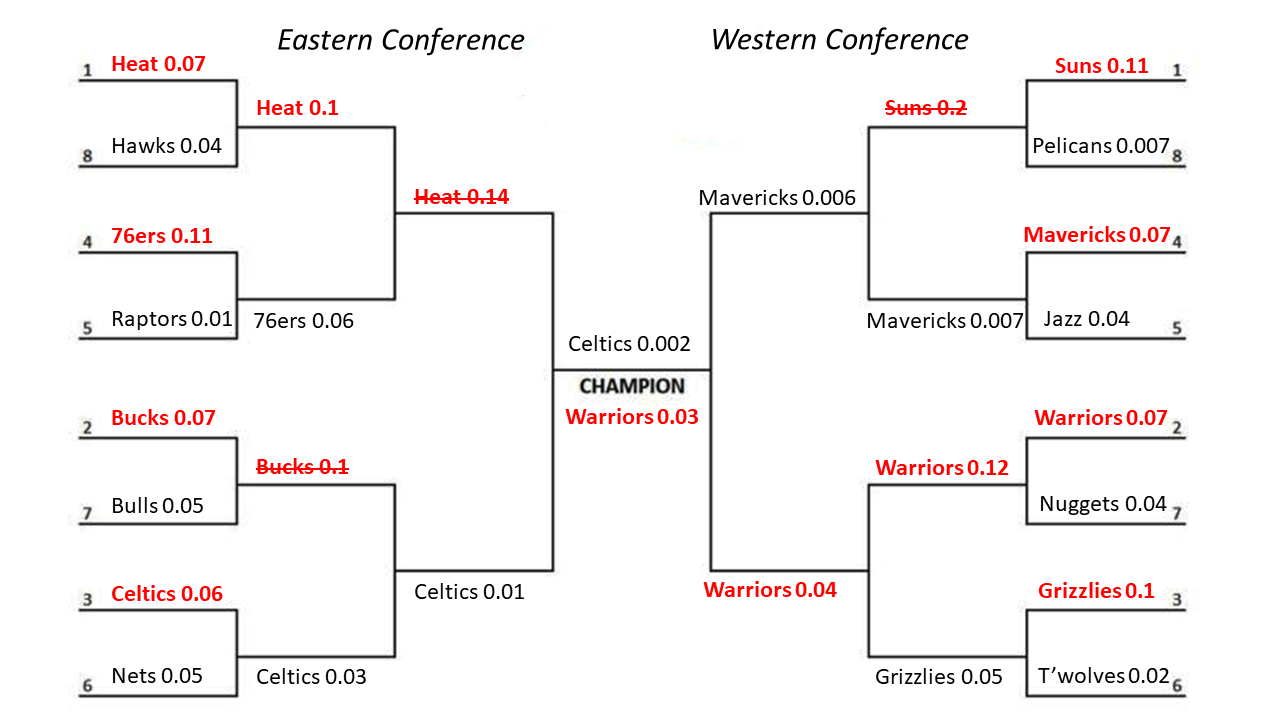
\includegraphics[width=\textwidth]{model/playoffs.png}
    \caption{playoff season 2021-2022}
    \label{fig:playoffSeason2022}
\end{figure}
\section{Conclusion}
The result in the figure \ref{fig:playoffSeason2022} predicts the result very well based on the statistics of the matches. These predictions could be further improved by adding player statistics, injuries, or playing strategies used in previous matches. 
\end{document}
